\chapter{実験}
\section{実験内容}
本論文において，共通実験は1つ，手法1は2つ，手法2は3つ，計6つの実験を設計実行した．
共通実験は体積測定精度の実験であり，\ref{sec:LiquidVolume}節の手法の精度を評価する実験である．
手法1の2つの実験は，注ぎ先の容器がテーブルに真っ直ぐまたは斜めに置かれた場合の精度を評価する実験である．
手法2はまず，表面張力の有無により2つの傾き角度と注いだ体積の関係の推測精度実験である．
次に，手法2の全体的な精度を評価する実験である．

\section{実験条件}
% 	\subsection{作業領域}\label{sec:workspace}
% 	ロボットアームの可動範囲により，注ぎ作業のできる範囲は
% 	手法1：300\,mm$\times$400\,mm程度である．
% 	手法2：200\,mm$\times$200\,mm程度である．
% 	図\ref{fig:WorkSpace}
% 	\begin{figure}[h]%TODO:作業領域の図
% 		\centering
% 		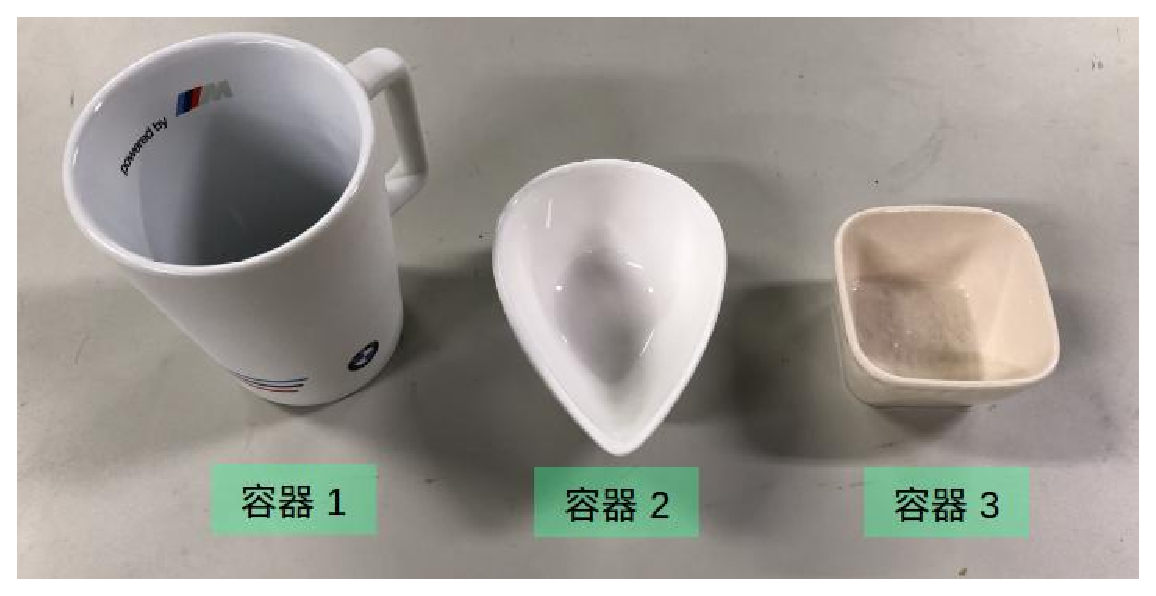
\includegraphics[width=0.4\linewidth]{fig/chp5/Cups-v2}
% 		\caption{作業領域}
% 		\label{fig:WorkSpace}
% 	\end{figure}

	\subsection{容器}
% 		\subsubsection{容器の識別}
% 		ロボットから見た右側の容器は注ぐ容器，左側は注ぎ先の容器である．
		
		\subsubsection{手法1に使用する容器}
		手法1の実験では，内容量が1000\,mlの牛乳パックから液体を別の容器に注いでいく．
		注ぐ目標容器として図\ref{fig:target-cups}に示す3つの容器を準備した．また，それぞれの体積は左から290\,ml，120\,ml，88\,mlである．
		\begin{enumerate}
		    \item 注ぐ容器：牛乳パック．
		    \item 注ぎ先の容器：容器1容器2と容器3．
		\end{enumerate}
		\begin{figure}[h]
			\centering
			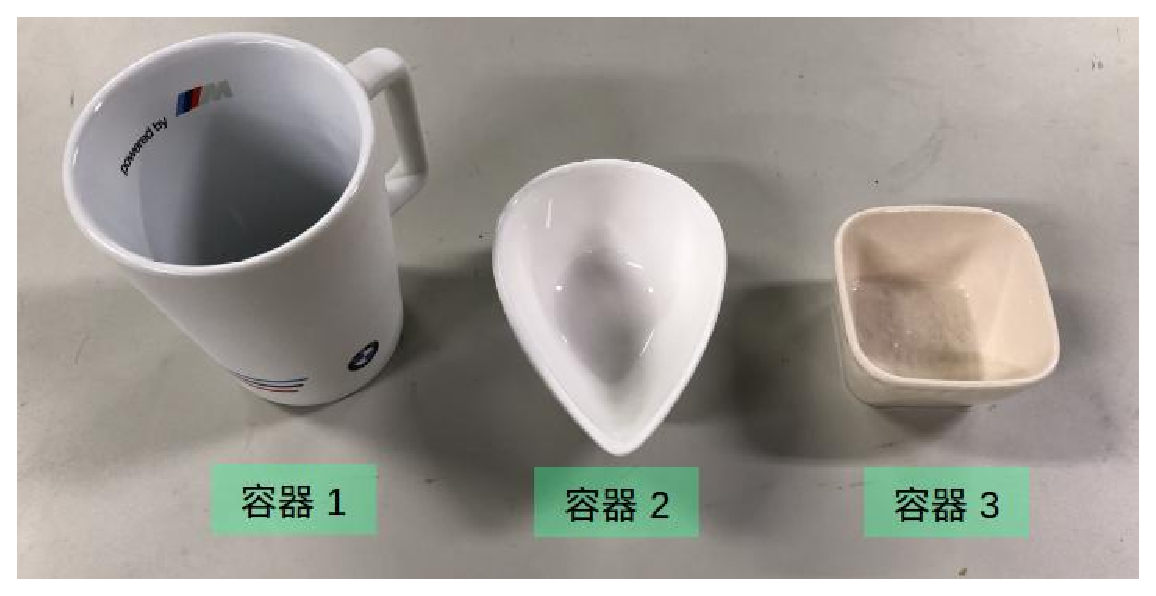
\includegraphics[width=0.8\linewidth]{fig/chp5/Cups-v2}
			\caption{手法1に使用する目標容器}
			\label{fig:target-cups}
		\end{figure}
	
		\subsubsection{手法2に使用する容器}
		手法2の実験では，以下の容器を使用した(図\ref{fig:Method2-Cups})．
		\begin{enumerate}
		    \item 注ぐ容器：容器3と容器4(半分に切った牛乳パック，容積355ml)．
		    \item 注ぎ先の容器：容器5(お皿)．
		\end{enumerate}
		\begin{figure}[h]
			\centering
			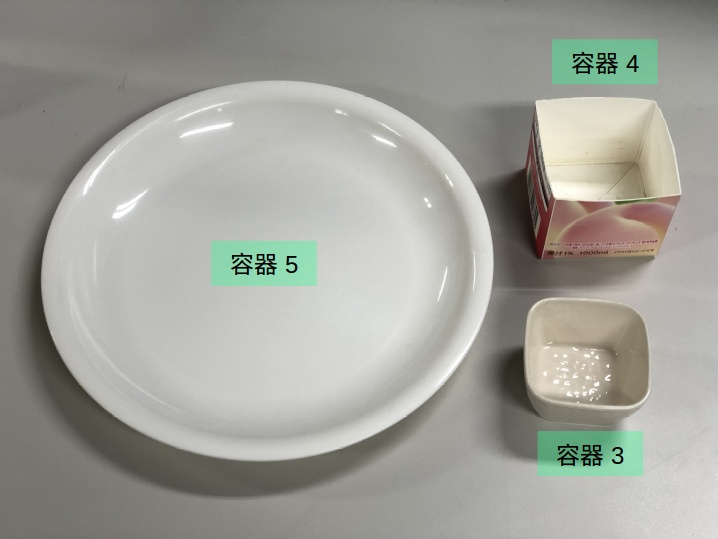
\includegraphics[width=0.6\linewidth]{fig/chp5/Method2-Cups}
			\caption{手法2に使用する注ぐ容器と目標容器である容器5}
			\label{fig:Method2-Cups}
		\end{figure}
	
	\subsection{目標容器体積真値の測定について}
	水道水の密度は約$1.000\mathrm{g/cm^3}$であり，目標容器の体積[ml]は数値的に目標容器に入った水道水の重量と等しい．
	測定方法はまず被測容器の中身を水と洗剤で洗い，清潔にする．
	また，水の表面張力をなくすため，洗剤を縁に薄く塗る．
	そして，水平に調整した秤に被測容器を乗せて，秤をゼロ表示にする．
	次に，水を入れながら液面を目視で確かめて，液面と被測容器の縁と平行になるまで注ぎ続ける．
	最後に，液面と被測容器の縁が平行した時の結果$m_\mathrm{water}$は
	\begin{equation}
	V_\mathrm{cup} = \rho_\mathrm{water} * m_\mathrm{water}
	\end{equation}
	で被測容器の体積を計算する．
	また，一つの容器に対し，三回測定した結果の平均を容器の体積とする．
	
	\subsection{ミルクティーの密度}
	今回，一部の実験(\ref{sec:exp-all}や\ref{sec:Method1Exp-1}や\ref{sec:Method1Exp-2}や\ref{sec:Method2-expAll}節)では，注ぐ液体としてミルクティーを使用した．
	実験では，注がれた液体の体積を重量から求めるが，使用したミルクティーの密度は未知であったため，予め測定を行った．
	
	ミルクティーの密度の測定方法は，容積が測定した容器にミルクティーを容器が満たされるまで注ぎ，重量の増加分から密度を計算した．
	このとき，液体の表面張力による誤差をなくすため，洗剤を縁に薄く塗った．
	最後は，液面と被測容器の縁が平行する時秤の結果$m_\mathrm{milktea}$は$\rho_\mathrm{milktea} = m_\mathrm{milktea} / V_\mathrm{cup}$式でミルクティーの密度を計算する．
	以上の手順により求められたミルクティーの密度は1.0276\,$\mathrm{g/cm^3}$であった．
	
	\subsection{秤について}
	重さの測定に使用した秤はTANITA製KD-320である．精度は表で示す．
	\begin{table}[h]
		\centering
		\caption{秤の精度}
		\begin{tabular}{@{}ccc@{}}
			\toprule 
			測定範囲 & 精度 \\ 
			\midrule
			0-300[g]&  0.1[g] \\ 
			0-1500[g]& 0.5[g] \\ 
			1500-3000[g]& 1.0[g] \\ 
			\bottomrule 
		\end{tabular} 
		\label{tab:Scaler}
	\end{table}
	
% 	\begin{figure}[h]%TODO:称的照片
% 		\centering
% 		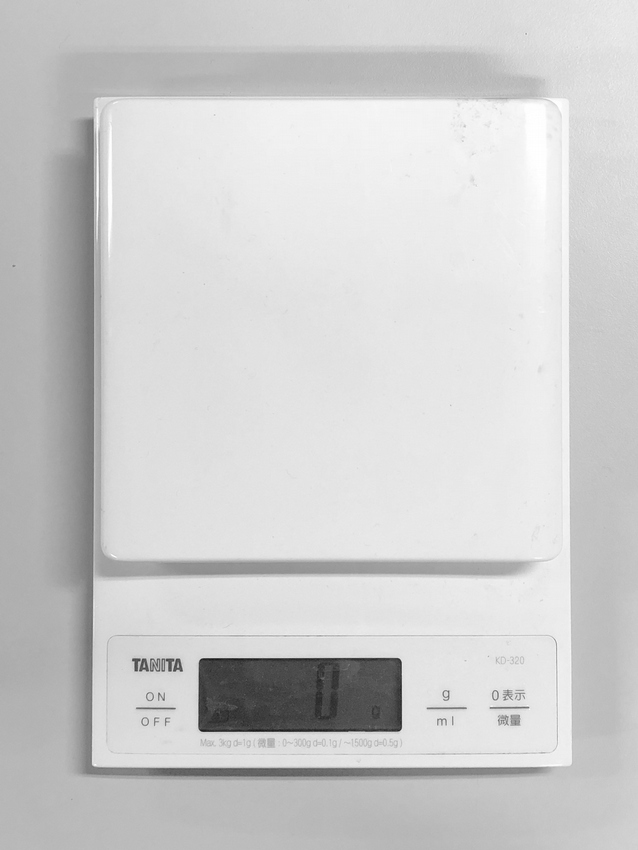
\includegraphics[width=0.6\linewidth]{fig/chp5/Scaler}
% 		\caption{使用した秤}
% 		\label{fig:scale}
% 	\end{figure}
	
	今回の手法1では，容器1を使用した際は0.5[g]の精度で計測し，容器2,3を使用した際には0.1[g]の精度で計測した．
	
	手法2では，測定範囲は全て300[g]以内であるため，0.1gの精度で計測した．	
	
\section{共通実験}
	\subsection{体積測定精度の実験}\label{sec:exp-all}
	この実験では，予め決められた体積の液体を入れ，
	\ref{sec:LiquidVolume}節で提案した手法で容器に注いだ液体の体積を推定することにより，体積測定精度を評価する．
	
		\subsubsection{実験方法}
		容器1に50\,mlから250\,mlまで50\,mlの間隔で液体を注ぎ，プログラムによって求められた推定値を記録する．
		実験は各体積に対して5回行い，推定値の平均と標準偏差を計算する．
		
		\subsubsection{実験結果}
		体積測定実験の結果を表\ref{Result0}に示す．
			\begin{table}[h]
				\centering
				\caption{体積測定精度の結果}
				\begin{tabular}{@{}ccc@{}}
					\toprule 
					実際の体積 & 推定値平均 & 標準偏差 \\ 
					\midrule
					50&  49.42 & 1.59 \\ 
					100&  100.34 & 2.05 \\ 
					150& 149.24 & 2.44 \\ 
					200& 198.8 & 3.78 \\ 
					250& 249.82 & 4.9 \\ 
					\bottomrule 
				\end{tabular} 
				
				\label{Result0}
			\end{table}
		
		\subsubsection{考察}
		推定された結果の平均値と標準偏差から，体積測定精度は実際の体積の2\%ほどであることが分かる．
		
\section{手法1の実験}
	\subsection{実験手順}\label{sec:Method1Exp-ProgramFlow}
	本項は手法1のプログラムの流れを紹介する．
	\begin{enumerate}
		\item テーブル全体を撮影し，牛乳パックと容器の位置を認識する．\\
% 		この撮影は固定した3つの位置で行う．
% 		また，その位置はテーブル全体を出来る限り撮影できるように選択される．
		\item 牛乳パック全体の点群を取得する．
		\item 牛乳パックの注ぎ口の方向を検出する．
		\item 左アームが牛乳パックの注ぎ口の方向を修正し，テーブルの中央へと移動させる．
		\item 右アームが牛乳パックを掴み，左アームの動作に支障のない位置へと移動させる．
	\end{enumerate}
	
	\vspace{3mm}
	\begin{enumerate}
		\setcounter{enumi}{5}
		\item 容器を上から撮影し，容器の方向と注ぎ位置$P_\mathrm{pour}$を検出する．
		\item 容器の方向に合わせて，容器の内部の点群$P_\mathrm{cup}$を取得する．
		\item 液面の高さから体積への変換テーブル$T$を作成する．\label{enum:TransformTable}
		\item 容器のAABBを計算する．\label{enum:calAABB}%TODO:Why？？
	\end{enumerate}
	
	\vspace{3mm}
	\begin{enumerate}
		\setcounter{enumi}{9}
		\item 左アームを注ぎ動作に干渉せずに容器の中身が見ることができる位置に移動する．\label{enum:pour-photographing}
		\item 右アームを注ぎ位置に移動させ，左アームのカメラで液面を検出しながら注ぐ．
	\end{enumerate}

	\subsection{注ぐ精度の評価実験1}\label{sec:Method1Exp-1}
	本実験では，目標容器をテーブルにまっすぐに置いたとき，指定した量を注げるか，その精度を評価する．
	
		\subsubsection{実験方法}
		3種類の容器に対して，それぞれ3通りの目標体積を設定し，注ぐ実験を行った．
		各容器・目標体積に対して，3回ずつの注ぎ作業を行った．
		容器のモデルは最初に一度だけ計測し，常に同じモデルを用いた．
		実験で用いた液体はミルクティーである．
		各動作ごとに秤で注がれた液体の重量を量り，ミルクティーの密度で割って体積へ変換した．
		目標体積は少量，中量，大量3つ選択された．
		具体的には，少量は容器の体積の0/3--1/3，中量は1/3--2/3，大量は2/3--3/3の範囲でランダムに選択した．
		
		\subsubsection{実験結果}
		実験の結果は，3回注いだ結果の標準偏差と平均誤差（結果の平均から目標値を引いたもの）で評価する．実験結果は表\ref{Result1}のとおりとなった．
		\begin{table}[h]
			\centering
			\caption{実験１の結果}
			\label{Result1}
			\begin{tabular}{@{}r rrr ccc@{}}
				\toprule
				目標値& \multicolumn{3}{c}{注いだ体積}& \multicolumn{2}{c}{分析}\\
				\cmidrule(lr){2-4} \cmidrule(lr){5-6}
				& \multicolumn{1}{c}{1} & \multicolumn{1}{c}{2} & \multicolumn{1}{c}{3}  & \multicolumn{1}{c}{標準偏差} & \multicolumn{1}{c}{平均誤差}\\
				\midrule
				容器1\\
				64 ml	&	65.2	&	65.7	&	66.2	&	0.50	&	1.70	\\
				178	ml	&	183.0	&	181.9	&	182.1	&	0.59	&	4.33	\\
				248 ml	&	252.0	&	252.5	&	253.0	&	0.50	&	4.50	\\
				容器2\\
				27 ml	&	26.2	&	26.9	&	26.5	&	0.35	&	-0.47	\\
				71 ml	&	67.8	&	67.1	&	68.6	&	0.75	&	-3.17	\\
				111 ml	&	104.4	&	104.6	&	103.7	&	0.47	&	-6.77	\\
				容器3\\
				12 ml	&	10.0	&	8.9		&	9.0		&	0.61	&	-2.70	\\
				41 ml	&	37.0	&	37.0	&	36.6	&	0.23	&	-4.13	\\
				71 ml	&	66.2	&	66.3	&	66.6	&	0.21	&	-4.63	\\
				\bottomrule
			\end{tabular}
		\end{table}
		
		\subsubsection{考察}%TODO:补全考察？
		この実験の考察は\ref{sec:Method1Exp-conclusion}節に書いた．
		
	\subsection{注ぐ精度の評価実験2}\label{sec:Method1Exp-2}
	本実験では，目標容器をテーブルに斜めに置いたとき，指定した量を注げるか，その精度を評価する．
	
		\subsubsection{実験方法}
		実験方法は，容器の置き方以外は実験1と同様である．
		ただし，容器には，底にテープでネジを固定し，テーブルに対して10度傾けて設置した．
		また，本実験では2/3--3/3の範囲の目標値はあふれる可能性があるため，実験を行わなかった．
		
		\subsubsection{実験結果}
		実験2の結果は，表\ref{Result2}のとおりとなった．
		\begin{table}[h]
			\centering
			\caption{実験2の結果}
			\label{Result2}
			\begin{tabular}{@{}r rrr cc@{}}
				\toprule
				目標値& \multicolumn{3}{c}{注いだ体積}& \multicolumn{2}{c}{分析}\\
				\cmidrule(lr){2-4} \cmidrule(lr){5-6}
				& \multicolumn{1}{c}{1} & \multicolumn{1}{c}{2} & \multicolumn{1}{c}{3}  & \multicolumn{1}{c}{標準偏差} & \multicolumn{1}{c}{平均誤差}\\
				\midrule
				容器1\\
				64 ml	&	63.7	&	63.7	&	64.7	&	0.58	&	0.03	\\
				178 ml	&	180.5	&	179.0	&	179.0	&	0.87	&	1.50	\\
				容器2\\
				27 ml	&	22.1	&	21.8	&	22.3	&	0.25	&	-4.93	\\
				71 ml	&	63.6	&	64.7	&	63.5	&	0.67	&	-7.07	\\
				容器3\\
				12 ml	&	8.9		&	8.4		&	9.2		&	0.40	&	-3.17	\\
				41 ml	&	36.9	&	37.0	&	37.1	&	0.10	&	-4.00	\\
				\bottomrule
			\end{tabular}
		\end{table}
	
		\subsubsection{考察}
		この実験の考察は\ref{sec:Method1Exp-conclusion}節に書いた．
		
	\subsection{考察}\label{sec:Method1Exp-conclusion}
	それぞれの実験の標準偏差の平均を見ると，立てて置いた際は0.47\,ml，斜めに置いた時は0.48\,mlであり，注ぎ動作の精度が高いことが分かった．
	しかし，平均誤差の標準偏差は，立てた場合は4.02\,ml，斜めにした場合は3.19\,mlであり，体積測定精度実験の結果をふまえると，注ぐシステムの誤差は主に体積の測定とモデルの精度によるものであると言える．
	
	それぞれの実験で，容器2に対して多くの液体を注ぐときの誤差が$-7\, \mathrm{ml}$程度と大きくなっている．
	この原因は，注いだ液体の体積が容器2の容積に近くなると，容器の縁と液面がつながり，一つの平面だと認識され，その結果，液面の高さが真値より高くなったため，注ぎ作業がより早く終わったことと考えられる．
	
	また，注ぎ動作最後の微調整段階では，注ぐ量が少なくなり，液体が目標容器に入らずに元の容器に沿ってこぼれてしまうことがある．
		
\section{手法2の実験}\label{sec:method2-exp}
	\subsection{注ぐ容器の傾き角度と注いだ体積の関係の推測精度実験1}\label{sec:method2-exp1}
	本実験では，傾き角度と注いだ体積の関係を推測するプログラムを抽出し，\ref{sec:pour-point-detect}と\ref{sec:angle-and-volume}節で提案したアルゴリズムの精度を評価する．
	また，本実験は容器3だけを使用する．
	
		\subsubsection{実験方法}
		一回の実験では，予め決めた体積の水を注ぐ容器に入れ，0度から注ぎ終わるまで5度の間隔で回転しつつ，各角度と注いだ水の体積を記録し，その結果を推測した傾き角度と注いだ体積の関係と比較する．

		具体的には：
		\begin{enumerate}
			\item 予め決めた体積の水を注ぐ容器に入れる．
			\item ロボットアームが注ぐ容器を掴み，注ぐ先容器の上に移動する．
			\item\label{enum:method2-exp1-a} 今の姿勢から，5度を加え，注ぐ方向に傾ける．
			\item 注いだ水の体積を秤で測る．
			\item\label{enum:method2-exp1-b} 上の結果を記録する．
			\item 液体が注ぎ終わるまで\ref{enum:method2-exp1-a}から\ref{enum:method2-exp1-b}までを繰り返す．
		\end{enumerate}
	
		そして，初期体積は，22[ml]，44[ml]や66[ml]とし，各初期体積に対して四回実験を実行した．
		また，注ぐ容器のモデルは手法2のアルゴリズムの精度を評価するため，容器内側のモデルを使用した．モデルの取得方法は\ref{sec:get-model}節手法1のパラメータを使用した方法である．モデルは毎回実験で取り直した．
		
		\subsubsection{実験結果}
		実験結果は図\ref{fig:method2-exp1-22}，\ref{fig:method2-exp1-44}，\ref{fig:method2-exp1-66}で示した．
		横軸は傾き角度[deg]，縦軸は体積[ml]である．
		黄色の線はアルゴリズムが推測した結果である．
		緑の線は実際に入れた体積である．
		青い線は推測と実際の差である．
		\begin{figure}[p]
			\centering
			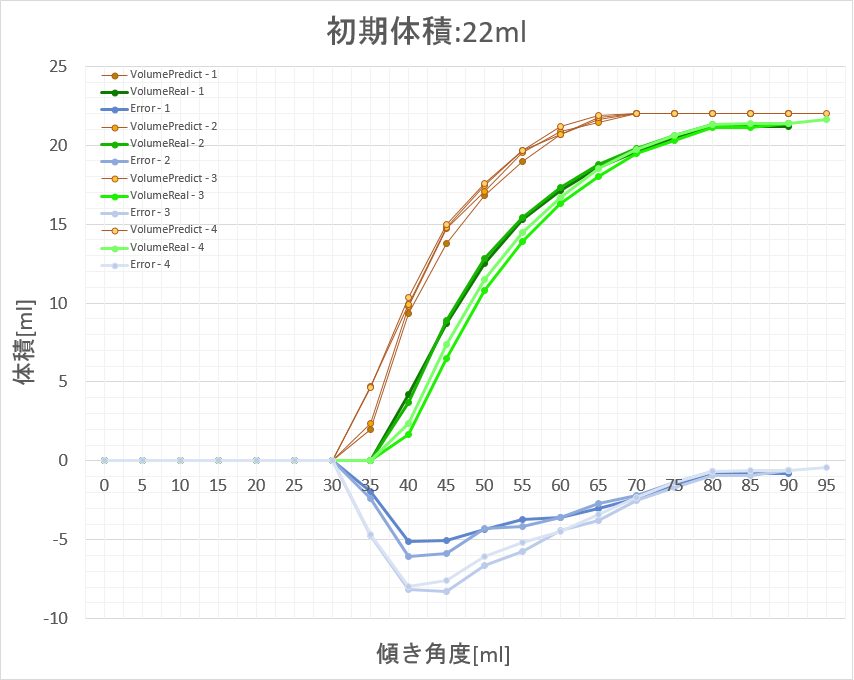
\includegraphics[width=0.9\linewidth]{fig/chp5/method2-exp1-22}
			\caption{手法2推測精度実験1-初期体積22[ml]}
			\label{fig:method2-exp1-22}
		\end{figure}
		\begin{figure}[p]
			\centering
			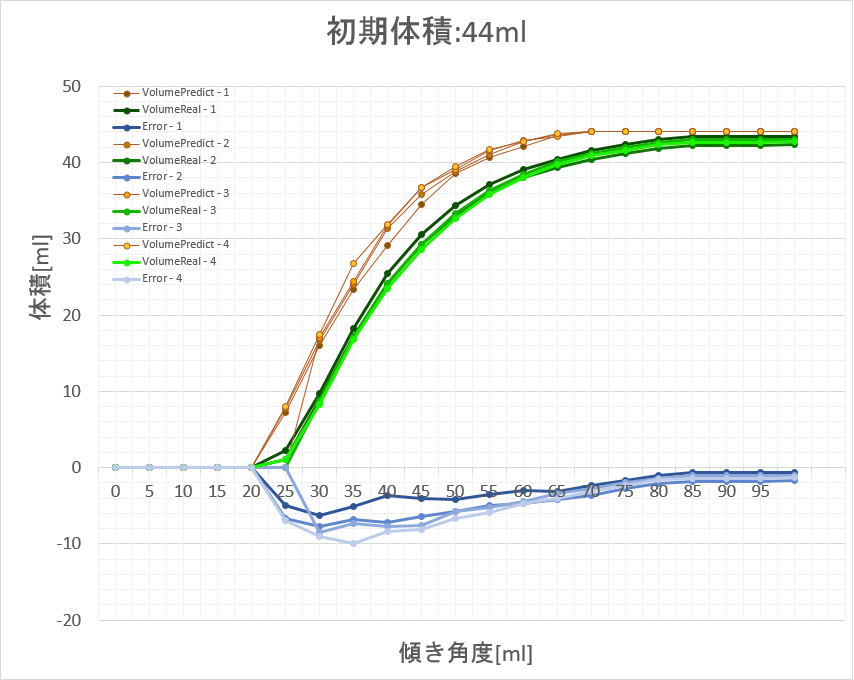
\includegraphics[width=0.9\linewidth]{fig/chp5/method2-exp1-44}
			\caption{手法2推測精度実験1-初期体積44[ml]}
			\label{fig:method2-exp1-44}
		\end{figure}
		\begin{figure}[p]
			\centering
			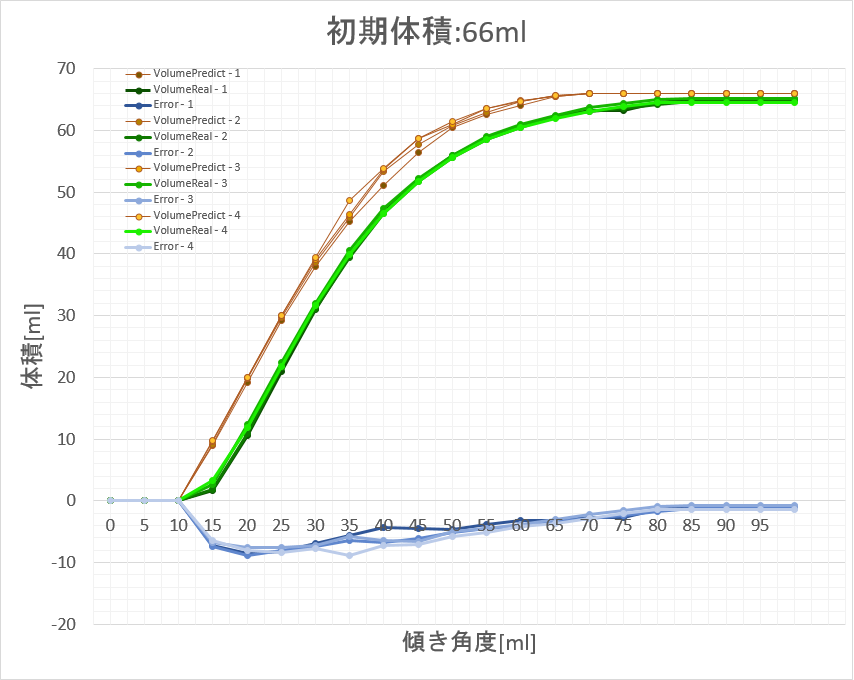
\includegraphics[width=0.9\linewidth]{fig/chp5/method2-exp1-66}
			\caption{手法2推測精度実験1-初期体積66[ml]}
			\label{fig:method2-exp1-66}
		\end{figure}
		
		\clearpage
		誤差に集中する：
		\begin{figure}[ht]
			\centering
			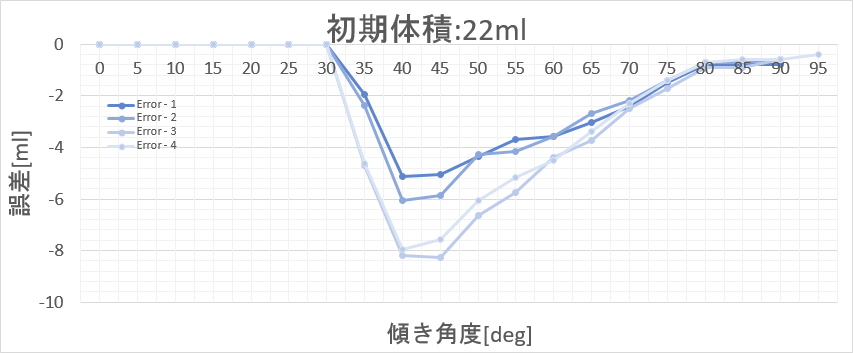
\includegraphics[width=1\linewidth]{fig/chp5/method2-exp1-22-error}
			\caption{手法2推測精度実験の誤差-初期体積22[ml]}
			\label{fig:method2-exp1-22-error}
		\end{figure}
		\begin{figure}[ht]
			\centering
			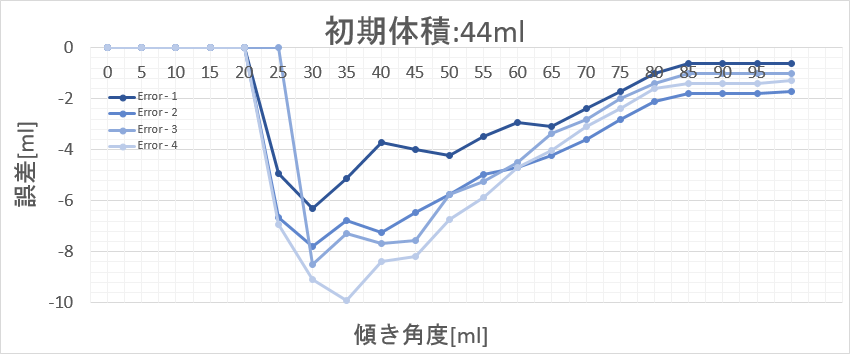
\includegraphics[width=1\linewidth]{fig/chp5/method2-exp1-44-error}
			\caption{手法2推測精度実験の誤差-初期体積44[ml]}
			\label{fig:method2-exp1-44-error}
		\end{figure}
	    \clearpage
		\begin{figure}[ht]
			\centering
			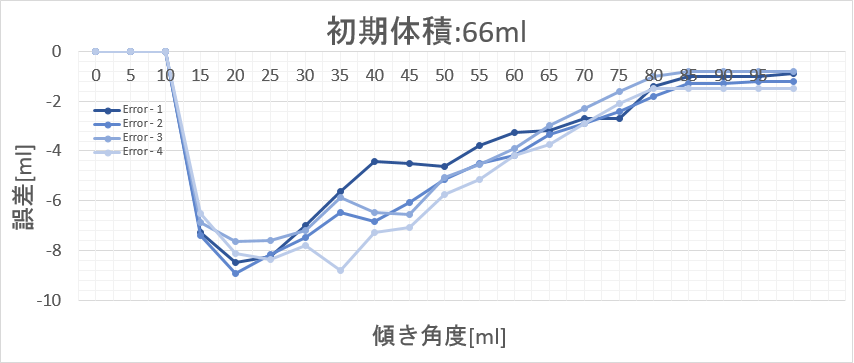
\includegraphics[width=1\linewidth]{fig/chp5/method2-exp1-66-error}
			\caption{手法2推測精度実験の誤差-初期体積66[ml]}
			\label{fig:method2-exp1-66-error}
		\end{figure}
	    
		\subsubsection{考察}
		結果から見ると，初期体積によらず，推測の誤差は注ぎ始めるところで-10[ml]から-5[ml]の幅に集中しており，注ぎ作業と共に減少していく．
		その誤差の原因は，下の図のような水と容器の表面張力の影響だと考えられる．
		
		\begin{figure}[h]
			\centering
			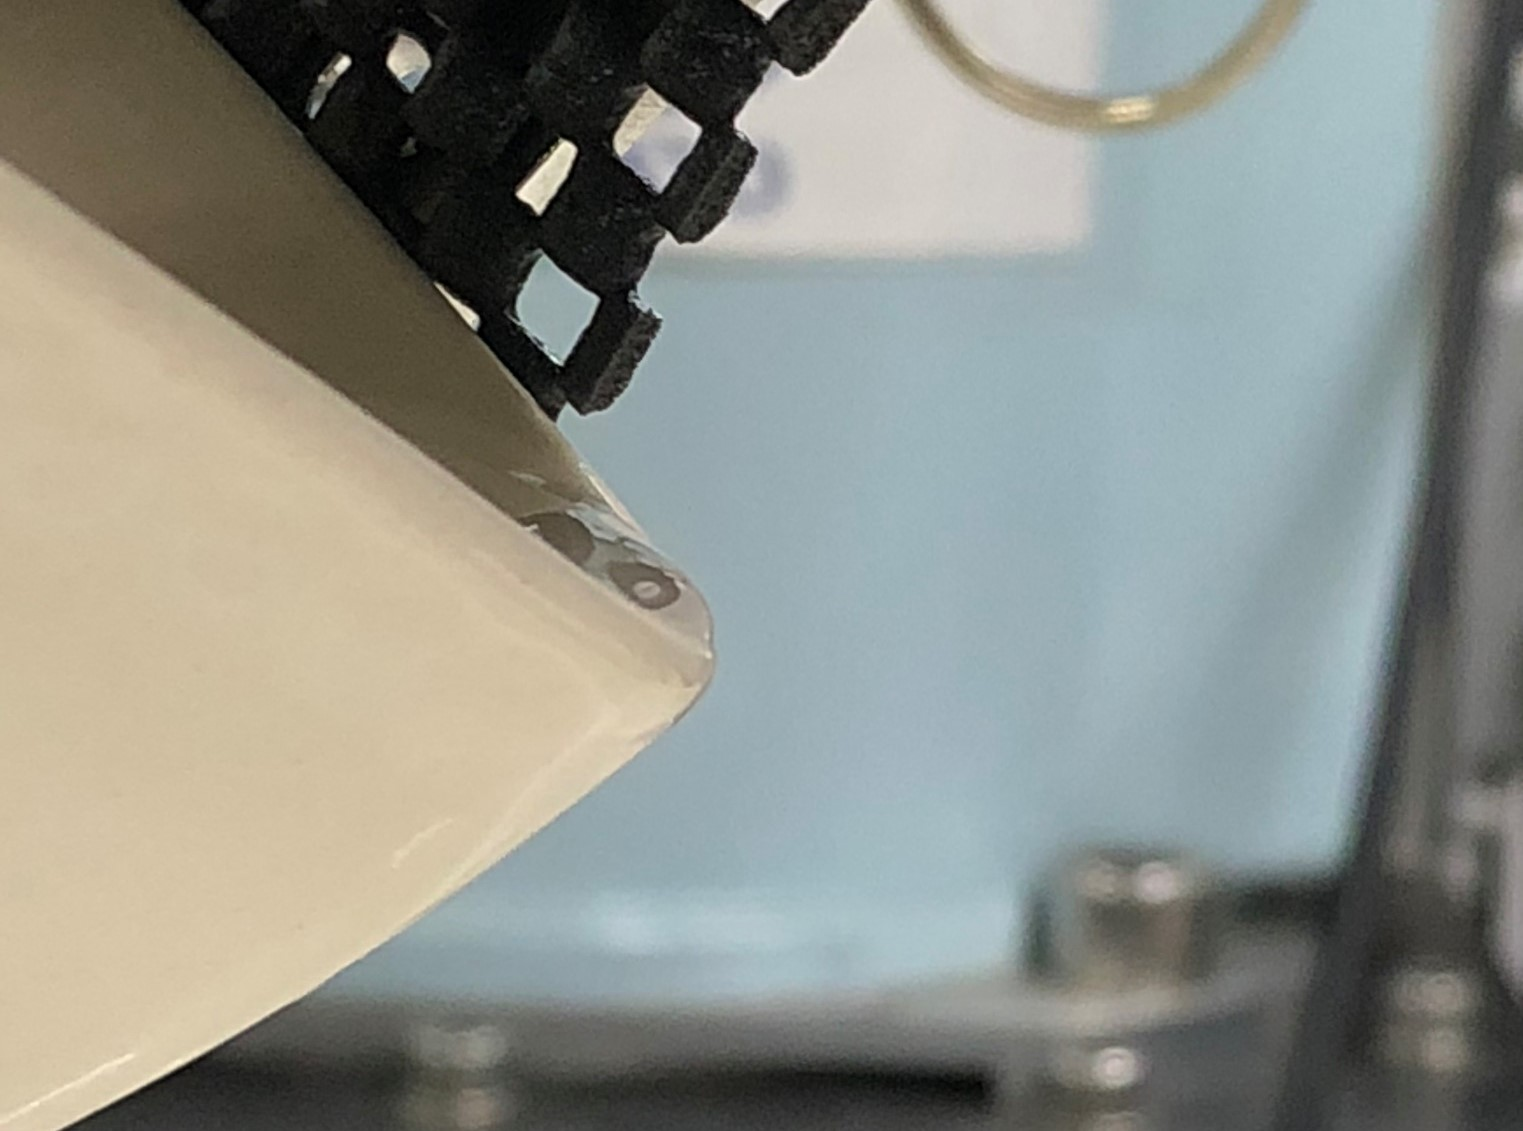
\includegraphics[width=0.5\linewidth]{fig/chp5/SurfaceTension}
			\caption{表面張力}
			\label{fig:SurfaceTension}
		\end{figure}
	
		図\ref{fig:SurfaceTension}により，注ぎ縁の付近において，液面はほぼ3[mm](定規で目視測定した)高くなってしまい，注いだ体積は推測より小さくなる．
		その誤差が徐々に減少していくことの原因は，注いでいるうちに液体と容器の縁の接触面積が徐々に減少し，表面張力も減少しているためだと考える．
		表面張力が弱くなると，液面は検出した注ぐポイントと近くなり，誤差も小さくなる．
		
	\subsection{注ぐ容器の傾き角度と注いだ体積の関係の推測精度実験2}\label{sec:method2-exp2}
	\ref{sec:method2-exp1}節の考察により，液体の流動は表面張力によって大きく妨げられる．
	そこで，アルゴリズムの精度を正しく評価するため，洗剤をコップの縁に塗布し，推測精度実験2を実施した．
	また，本実験も容器3だけを使用する．
	
		\subsubsection{実験方法}
		実験方法は\ref{sec:method2-exp1}節の方法や手順と同じである．
		ただし，初期体積は[3/4]に固定した．
		
		\subsubsection{実験結果}
		実験結果は図\ref{fig:method2-exp2-66-NoSurfaceTension}で示した．
		\begin{figure}[p]
			\centering
			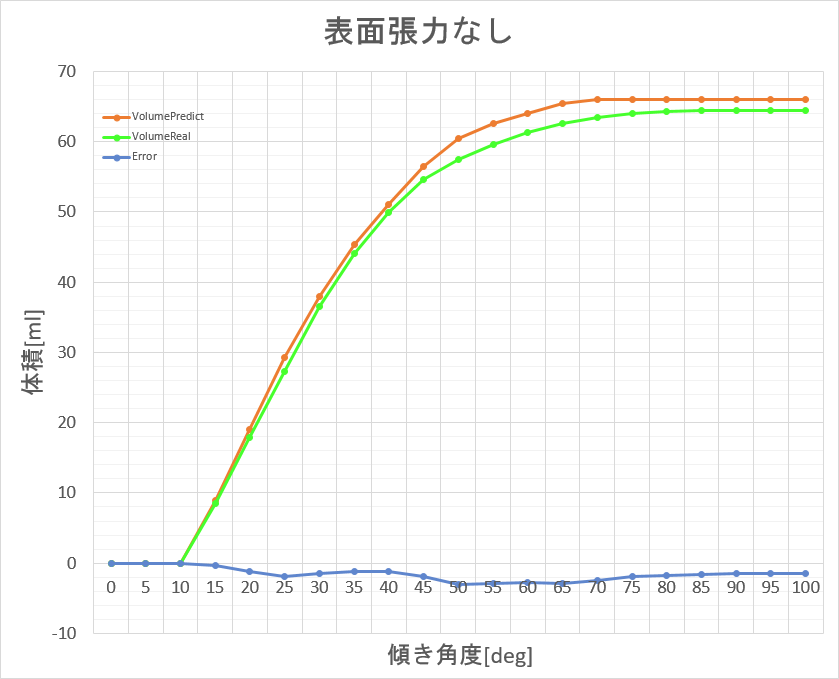
\includegraphics[width=0.9\linewidth]{fig/chp5/method2-exp2-66}
			\caption{手法2推測精度実験-表面張力なし}
			\label{fig:method2-exp2-66-NoSurfaceTension}
		\end{figure}
	
	    \clearpage
		\subsubsection{考察}
		洗剤を使用した結果は図\ref{fig:NoSurfaceTension}のように：
		\begin{figure}[h]
			\centering
			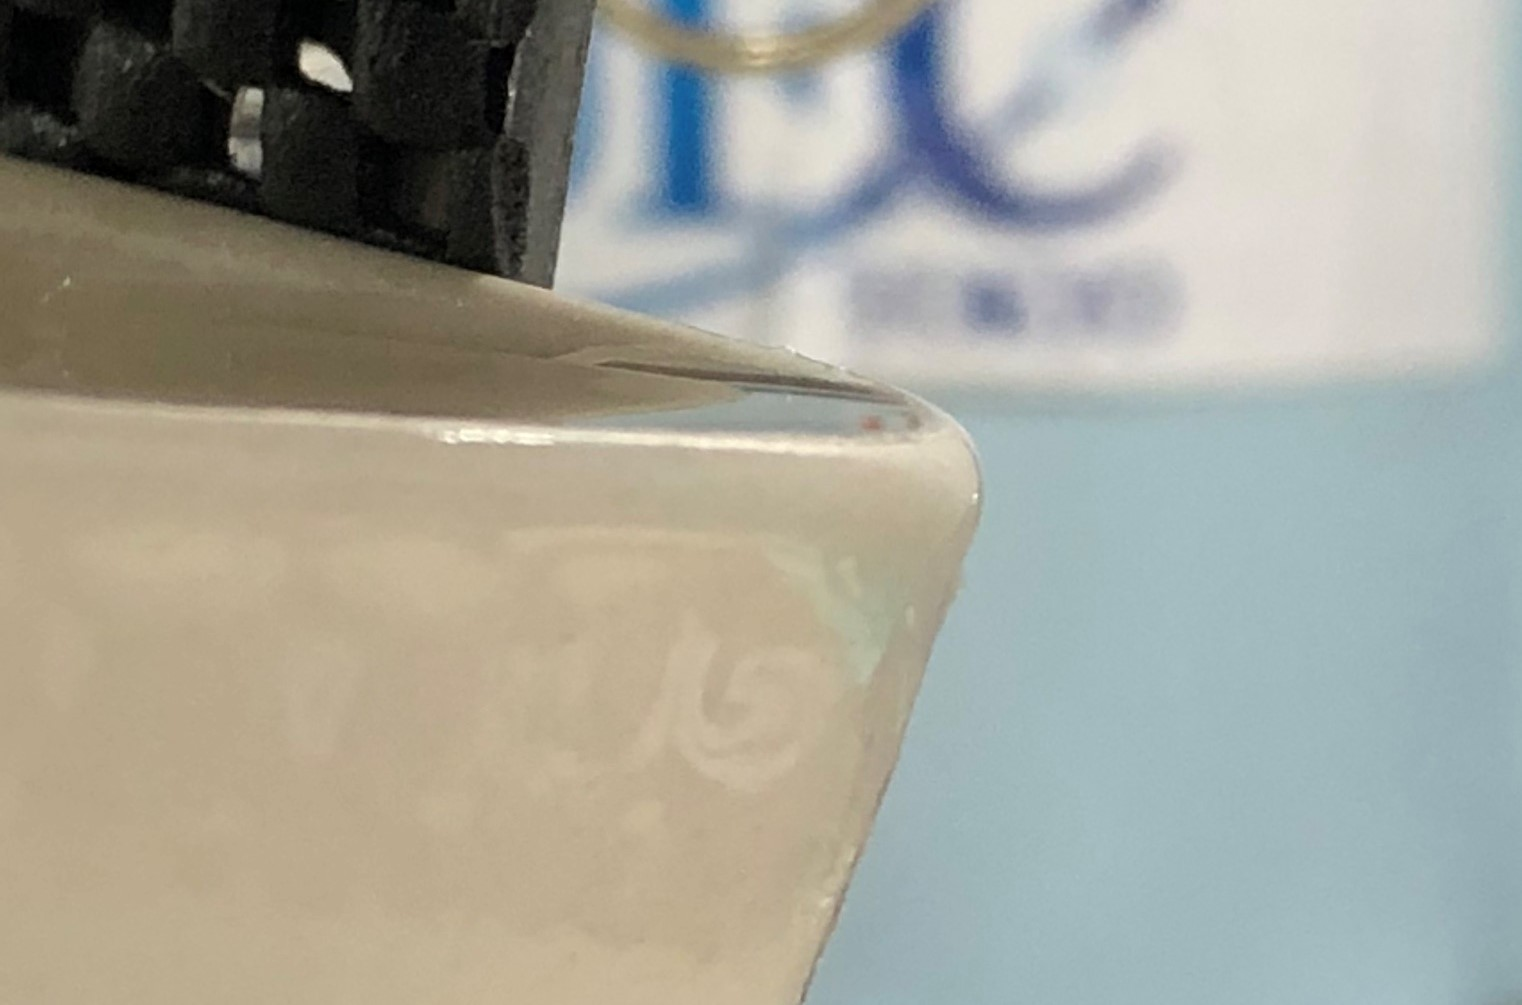
\includegraphics[width=0.5\linewidth]{fig/chp5/NoSurfaceTension}
			\caption{表面張力なし}
			\label{fig:NoSurfaceTension}
		\end{figure}
	
		図\ref{fig:method2-exp2-66-NoSurfaceTension}と\ref{fig:NoSurfaceTension}により，表面張力の影響はほとんどなくなった．
		
		実験の結果について，表面張力の影響がないと，誤差の平均は1.57，標準偏差は0.93である．
		実験\ref{sec:method2-exp1}より，誤差が大きく減少した．
		2つ実験の誤差を比較すると，表面張力の影響は最大10[ml]程度と分かった．
		
% 	%TODO:これから未完成です．
% 	\subsection{手法2注ぎ制御精度の評価実験}\label{sec:Method2-exp-accur}
% 	本実験は手法2の制御方法の精度を評価する．
	
	
% 		\subsubsection{実験方法}
% 		注ぐ容器モデルを取得することやその中の液体初期体積を測定することは全部プログラムに書き込む．
% 		\subsubsection{実験結果}
% 		\subsubsection{考察}
		
	\subsection{手法2注ぐ精度の評価実験}\label{sec:Method2-expAll}
	本実験では，両方の容器をテーブルにまっすぐに置いたとき，指定した量を注げるか，その精度を評価する．
	また，本実験は容器3だけを使用する．
		
		\subsubsection{実験方法}
		一回の実験は注ぐ容器のモデルを取得し，変換テーブルを計算し，容器3に対して，
		0[ml]から65[ml]まで5[ml]の間隔(容器4は0[ml]〜230[ml]，10[ml]の間隔)で段階的に注ぎ，注いだ体積を記録する．
		初期体積について，容器3は65[ml]以上，容器4は230[ml]以上容器の容積までの範囲内でランダムに選択した．容器3と容器4はそれぞれ4回実験を行った．
		
		具体的には：
    		\begin{enumerate}
    		\item テーブル全体を撮影し，注ぐ容器の位置を認識する．
        	\item \ref{sec:get-model}節の方法で，注ぐ容器のモデルを取得するための撮影位置を計算する．
        	\item 計算した位置で，撮影した点群を合成し，モデルを作成する．
    		\item 注ぐ容器を上から撮影することで初期液面の高さを検出し，初期液体の体積を計算する．
    		\item \ref{sec:pour-point-detect}の方法で注ぐポイントを検出し，\ref{sec:Method2-TableCal}節の方法で傾き角度から目標体積への変換テーブルを作成する．
    		\item 変換テーブルで，注ぎ作業を行う．
    		\end{enumerate}
    				
		また，本実験は表面張力を排除しないまま，実験を行った．
    	
		\subsubsection{実験結果}
		容器3の結果は図\ref{fig:method2-exp3-Cup4-All}で，目標体積への誤差は図\ref{fig:method2-exp3-Cup4-Error}で示した．
		容器4の結果は図\ref{fig:method2-exp3-CupMilk-All}で，目標体積への誤差は図\ref{fig:method2-exp3-CupMilk-Error}で示した．
    		\begin{figure}[p]
    			\centering
    			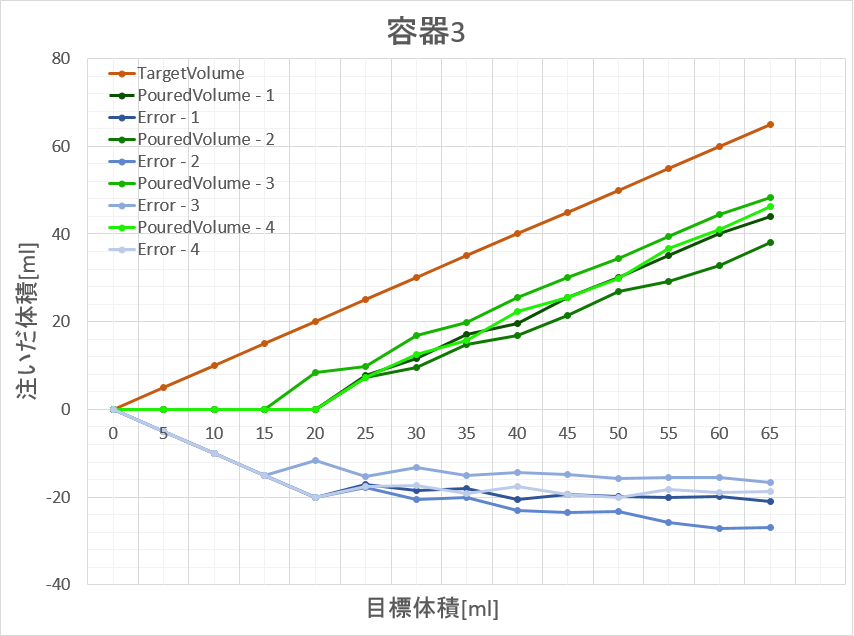
\includegraphics[width=0.9\linewidth]{fig/chp5/method2-exp3-Cup4-All}
    			\caption{手法2注ぐ精度の結果-容器3}
    			\label{fig:method2-exp3-Cup4-All}
    		\end{figure}
    		\begin{figure}[hp]
    			\centering
    			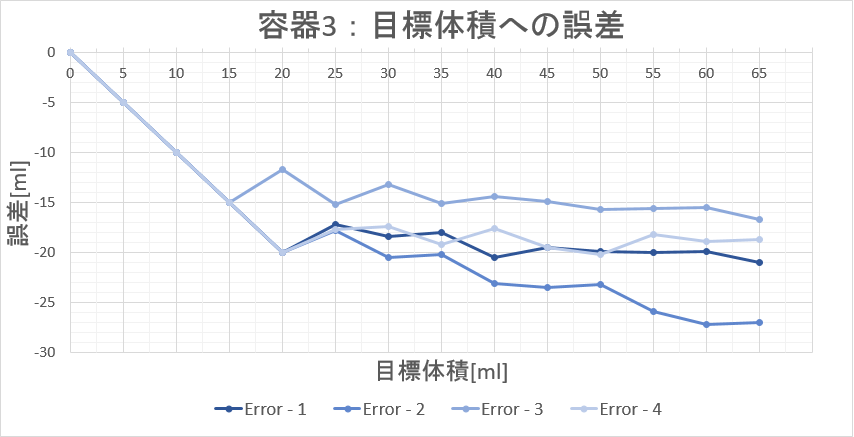
\includegraphics[width=0.9\linewidth]{fig/chp5/method2-exp3-Cup4-Error}
    			\caption{手法2注ぎ作業の誤差-容器3}
    			\label{fig:method2-exp3-Cup4-Error}
    		\end{figure}
    		\begin{figure}[p]
    			\centering
    			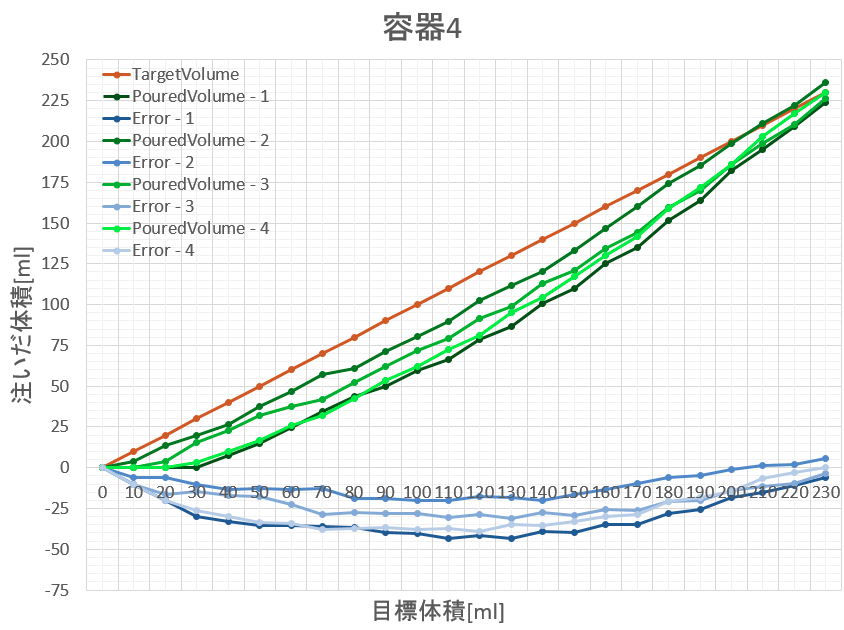
\includegraphics[width=0.9\linewidth]{fig/chp5/method2-exp3-CupMilk-All}
    			\caption{手法2注ぐ精度の結果-容器4}
    			\label{fig:method2-exp3-CupMilk-All}
    		\end{figure}
    		\begin{figure}[hp]
    			\centering
    			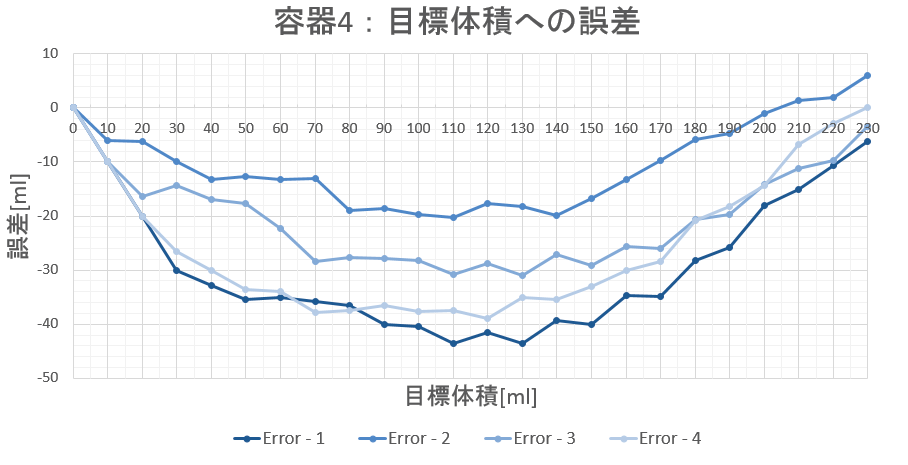
\includegraphics[width=0.9\linewidth]{fig/chp5/method2-exp3-CupMilk-Error}
    			\caption{手法2注ぎ作業の誤差-容器4}
    			\label{fig:method2-exp3-CupMilk-Error}
    		\end{figure}
		\subsubsection{考察}
        容器3の実験誤差に対して，平均-15.68[ml]，標準偏差は6.51[ml]であった．
        容器4の実験誤差に対して，平均-25.90[ml]，標準偏差は12.33[ml]であった．
        手法2の精度が手法1より大幅に低いことが分かった．
        
        容器3の結果について，誤差の原因(影響が大きい順)は
        	\begin{enumerate}
    		\item 取得した注ぐ容器のモデルの誤差．
    		\item 表面張力．
    % 		\item 傾き角度と注いだ体積の関係を推測する時の注ぐ方向と実際の注ぐ方向が違う．
		    \end{enumerate}
		1について，容器の容積に影響するのは容器内部の形状である．
		また，手法2は容器内側の点群モデルを使用すると精度が良くなる．
		しかし，現実は容器内部の点群が，容器に入った液体が原因で取得不能になる．
		そこで，内側点群の代わりに外側の点群が使用された．
		つまり，外側の点群から容器モデルを作ると，手法2の精度は容器の厚さに影響される．
		今回の容器3の厚さは注ぎ縁が3[mm]で，容器の底が7[mm]であり，厚さの影響は大きいと考えられる．
		2について，手法2の傾き角度と注いだ体積の関係の推測精度を知るための2つの実験(\ref{sec:method2-exp1}節と\ref{sec:method2-exp2}節)の結論により，表面張力の影響は容器3に対して，最大10[ml]程度である．
    % 		3について，手法2の傾き角度と注いだ体積の関係は注ぐ方向に敏感する．
    % 		つまり，容器3に対して，注ぐ方向が対角線にする時と中心線にする時，傾き角度と注いだ体積の関係は大幅に違う．
    		
        容器4の結果について，誤差の原因(影響が大きい順)は
        \begin{enumerate}
		\item 容器4の材質の柔軟さによる変形．
		\item 表面張力．
		\item 取得した注ぐ容器のモデルの誤差．
% 		\item 傾き角度と注いだ体積の関係を推測する時の注ぐ方向と実際の注ぐ方向が違う．
		\end{enumerate}
		1について，容器4は紙容器のため，グリッパの閉じる力により変形しやすい．
		その変形により，傾き角度と注いだ体積の関係を推測する際に使用されるモデルと実際に使う容器との形状の差異が発生し，誤差が生じると考えられる．
		2について，容器3の誤差分析と同じである．
		しかし，容器4の液面面積は容器3より大きいため，表面張力が同じでも，誤差の大きさは容器4のほうが大きいと考えられる．
		3について，容器4の厚さの影響は前の2つの原因より小さいが，容器4底部の形が複雑なため，少々誤差が出る．
		容器4の厚さは注ぎ縁が0.6[mm]で，容器の底が0.6[mm]から3[mm]である．
        
    \subsection{考察}  
    手法2の全体から見ると，誤差の平均は20.79[ml]であることが分かった．
    実験\ref{sec:Method2-expAll}の考察により，手法2の精度に影響する要因は表面張力とモデルの誤差である．
    そして紙コップのような容器に対しては，更に変形による誤差も要因となる．
        
\section{考察}
2つの手法を比較すると，手法1は手法2より遥かに精度が良いことが分かった．
手法1の利点は注ぎ先の容器の内側モデルを使用可能なことであり，更にリアルタイムに注いだ体積を計算し，フィードバックできる点である．

% 手法1は手法2の精度を影響する要因の2つを全部なくした．

